\documentclass[UTF8]{ctexart}
\usepackage{mathtools,wallpaper}
\usepackage{listings}
\usepackage{t1enc}
\usepackage{pagecolor}
\usepackage{geometry}
\usepackage{diagbox}
\usepackage{CJK}
\usepackage{graphicx}
\usepackage{wrapfig}
\usepackage{amssymb}
\newcommand{\song}{\CJKfamily{song}}
\newcommand{\xiaoer}{\fontsize{18pt}{18pt}\selectfont}
\newcommand{\sanhao}{\fontsize{16pt}{16pt}\selectfont}
\newcommand{\sihao}{\fontsize{14pt}{24pt}\selectfont}
\geometry{left=2cm,right=2cm}

\linespread{1.7}
\geometry{left=3.18cm,right=3.18cm,top=2.54cm,bottom=2.54cm}
\setlength{\parindent}{0pt}
\begin{document}
\CTEXsetup[format={\Large\bfseries}]{section}
\begin{center}
    \song\xiaoer\textbf{中国科学技术大学计算机学院} \\
    \song\xiaoer\textbf{《数字电路实验》报告} \\
    \ \\
    \ \\
    \ \\
    
\includegraphics{school.jpg} \\
    \ \\
    \ \\
    \song\sanhao 实验题目:简单组合逻辑电路 \\
    \song\sanhao 学生姓名:徐亦昶\\
    \song\sanhao 学生学号:PB20000156\\
    \song\sanhao 完成日期:2021.11.7\\
    \ \\
    \ \\
    \song\sihao 计算机实验教学中心制 \\
    \song\sihao 2020年09月
\end{center}
\newpage
\song\sihao
【实验题目】
\newline
简单组合逻辑电路
\newline
【实验目的】
\begin{enumerate}
    \item 熟练掌握 Logisim 的基本用法
    \item 进一步熟悉 Logisim 更多功能
    \item 用 Logisim 设计组合逻辑电路并进行仿真
    \item 初步学习 Verilog 语法
\end{enumerate}
\newline
【实验环境】
\newline
\begin{enumerate}
    \item PC一台,能流畅的连接校园网
    \item Logisim 仿真工具
    \item vlab平台
\end{enumerate}
【实验过程】
\newline
Step 1:用真值表自动生成电路
\newline
1、摆放引脚
\newline
\begin{figure}[h!]
    \centering
    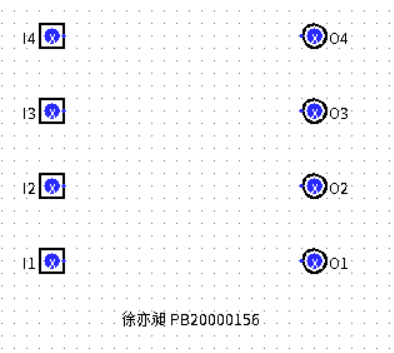
\includegraphics{S1_1.PNG}
    \caption{Step1 引脚摆放}
\end{figure}
2、设置真值表并生成电路
\newline
\begin{figure}[h!]
    \centering
    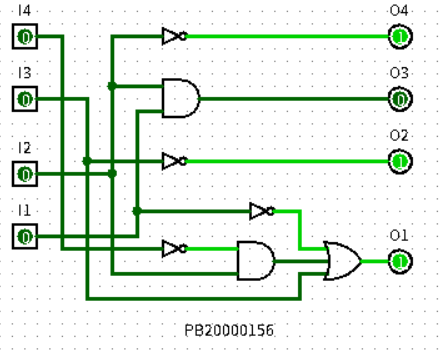
\includegraphics{S1_2.PNG}
    \caption{Step1 电路图}
\end{figure}
\newline
Step 2:用表达式生成电路图
\newline
1、输入表达式并进行化简(图中仅以一个输出变量为例)
\newline
\begin{figure}[h!]
    \centering
    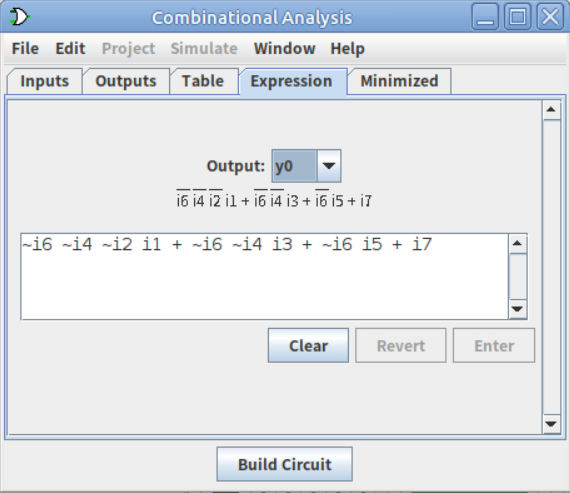
\includegraphics{S2_2.PNG}
    \caption{Step2 化简}
\end{figure}
2、生成电路
\newline
\begin{figure}[h!]
    \centering
    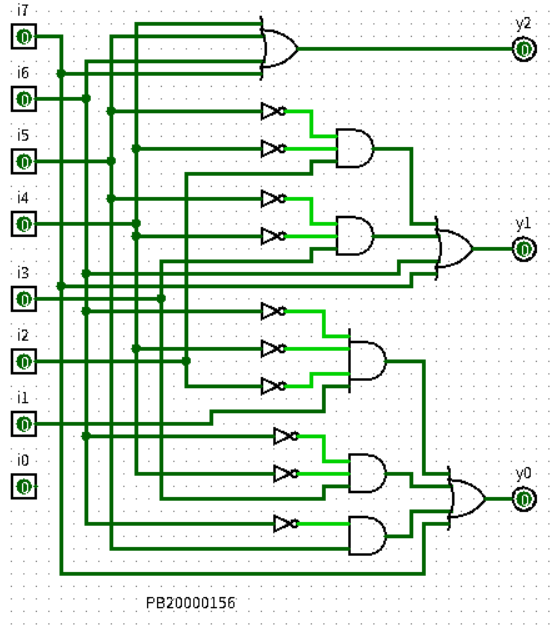
\includegraphics{S2_1.PNG}
    \caption{Step2 电路图}
\end{figure}
3、统计电路的基本信息
\newline
\begin{figure}[h!]
    \centering
    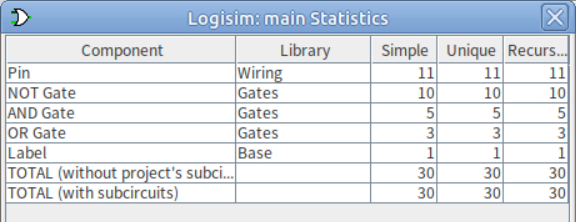
\includegraphics{S2_3.PNG}
    \caption{Step2 统计}
\end{figure}
Step 3:Verilog HDL 语法入门
\newline
这里主要总结从示例代码学到的东西。
\begin{enumerate}
    \item 一个模型用module定义,相当于javascript中的function。函数名后的括号中包括输入、输出,注意括号后要跟分号(这一点和C语言不一样)。那么如何表示模块的终止呢?在代码结束处使用关键字endmodule。
    \item 输入使用input,输出使用output,后面跟变量名。
    \item 可以使用assign语句赋值。
    \item 注释及基本的逻辑运算符和C语言相同。
    \item 大括号表示位的联结,比如\{a,b\}表示将a和b这两个bit联结成位数更大的2-bit。
    \item 电路中用于传递中间结果的线可以用wire定义。
    \item 可以对已定义模型进行复用,格式为:<模型名> <实例名>(参数1,参数2,...,参数n)或<模型名> <实例名>(.形参1(参数1),.形参2(参数2),...,.形参n(参数n))。第二种是对应端口赋值,比起第一种易读。
\end{enumerate}
【实验练习】
\newline
题目1:
\newline
\begin{figure}[h!]
    \centering
    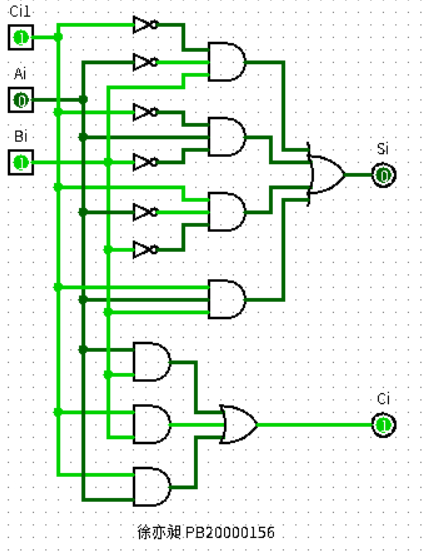
\includegraphics{p1.PNG}
    \caption{题目1}
\end{figure}
\newpage
题目2:
\newline
小tip:键盘长按可以快速输入,不需要一直点。
\newline
\begin{figure}[h!]
    \centering
    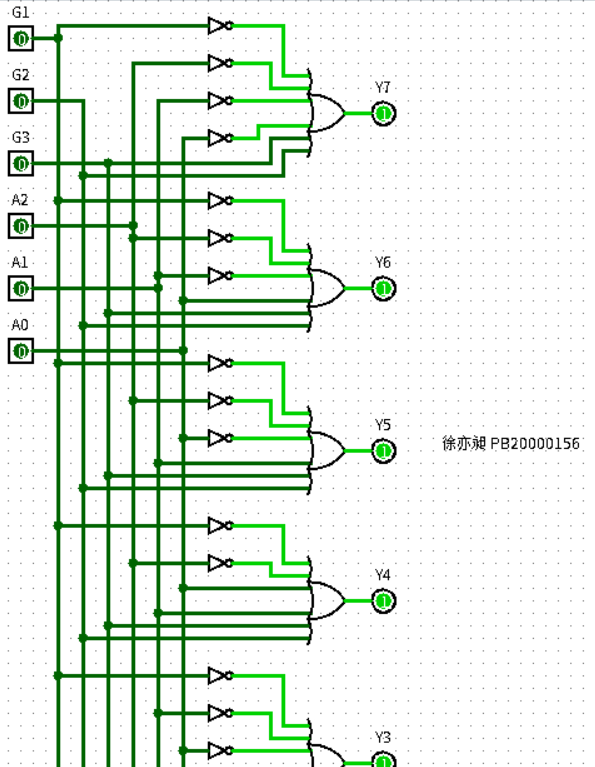
\includegraphics{p2_1.PNG}
    \caption{题目2}
\end{figure}
\newpage
\begin{figure}[h!]
    \centering
    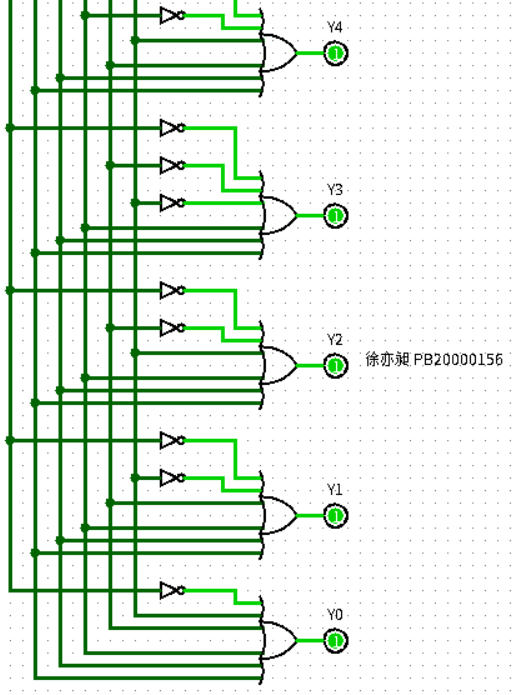
\includegraphics{p2_2.PNG}
    \caption{题目2(续)}
\end{figure}
\newpage
题目3:
\newline
\begin{figure}[h!]
    \centering
    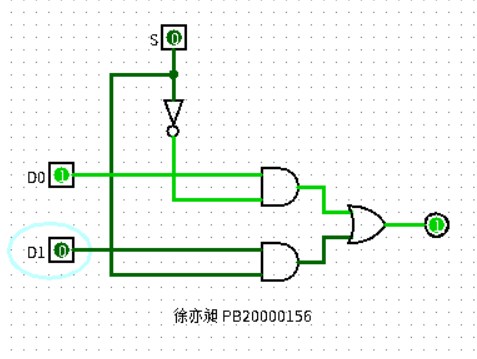
\includegraphics{p3.PNG}
    \caption{题目3 电路图}
\end{figure}
\begin{lstlisting}[language={Verilog},numbers=left,numberstyle=\tiny,%frame=shadowbox,  
    rulesepcolor=\color{red!20!green!20!blue!20},  
    keywordstyle=\color{blue!70!black},  
    commentstyle=\color{blue!90!},  
    basicstyle=\ttfamily]
module mux2to1_dataflow(
    input a,b,sel,
    output out);
assign out=(a & ~sel) | (b & sel);
endmodule
\end{lstlisting}
题目4:
\newline
\begin{figure}[h!]
    \centering
    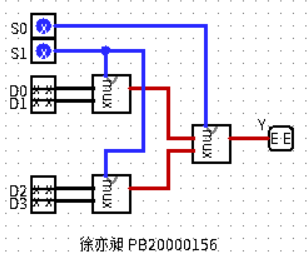
\includegraphics{p4.PNG}
    \caption{题目4 电路图}
\end{figure}
\begin{lstlisting}[language={Verilog},numbers=left,numberstyle=\tiny,%frame=shadowbox,  
    rulesepcolor=\color{red!20!green!20!blue!20},  
    keywordstyle=\color{blue!70!black},  
    commentstyle=\color{blue!90!},  
    basicstyle=\ttfamily]
    module mux2to1_dataflow(
        input a,b,sel,
        output out);
    assign out=(a & ~sel) | (b & sel);
    endmodule
    
    module mux4to1_dataflow(
        input a,b,c,d,sel1,sel0,
        output out);
    wire Y0,Y1;
    mux2to1_dataflow mux_inst1(
        .a (a),
        .b (b),
        .sel (sel0),
        .out (Y0));
    mux2to1_dataflow mux_inst2(
        .a (c),
        .b (d),
        .sel (sel0),
        .out (Y1));
    mux2to1_dataflow mux_inst3(
        .a (Y0),
        .b (Y1),
        .sel (sel1),
        .out (out));
    endmodule
\end{lstlisting}
题目5:
\newline
\begin{lstlisting}[language={Verilog},numbers=left,numberstyle=\tiny,%frame=shadowbox,  
    rulesepcolor=\color{red!20!green!20!blue!20},  
    keywordstyle=\color{blue!70!black},  
    commentstyle=\color{blue!90!},  
    basicstyle=\ttfamily]
    module encoder(
        input i7,i6,i5,i4,i3,i2,i1,
        output y2,y1,y0);
    assign y2 = i7 | ~i7 & i6 | ~i7 & ~i6 & i5 | ~i7 & ~i6 & ~i5 & i4;
    assign y1 = i7 | ~i7 & i6 | ~i7 & ~i6 & ~i5 & ~i4 & i3 | ~i7 & ~i6 & ~i5 & ~i4 & ~i3 & i2;
    assign y0 = i7 | ~i7 & ~i6 & i5 | ~i7 & ~i6 & ~i5 &~i4 & i3 | ~i7 & ~i6 & ~i5 & ~i4 & ~i3 & ~i2 & i1;
    endmodule
\end{lstlisting}
题目6:
\newline
使用Losgisim根据逻辑表达式建图的功能生成如下电路图:
\newline
\begin{figure}[h!]
    \centering
    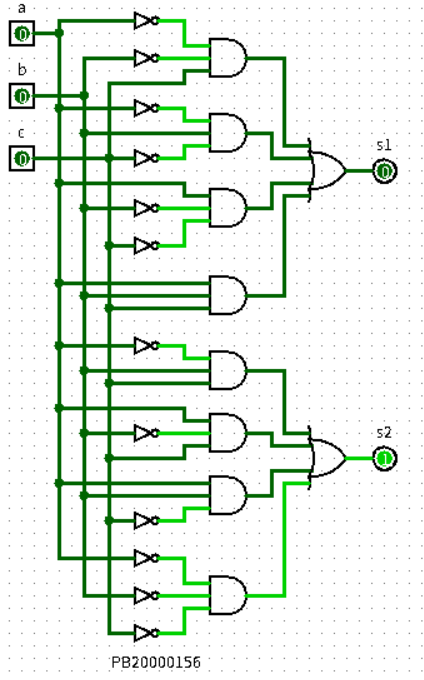
\includegraphics{p6_1.PNG}
    \caption{题目6 电路图}
\end{figure}
查看真值表:
\begin{figure}[h!]
    \centering
    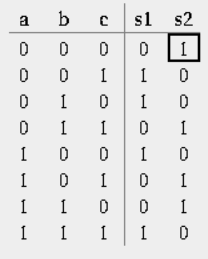
\includegraphics{p6_2.PNG}
    \caption{题目6 真值表}
\end{figure}
可以看出这是一个奇偶校验的电路s1指示1的个数是否为奇数,s2指示1的个数是否为偶数。
【总结与思考】
\newline
1、通过本次实验,掌握了除手动搭建电路以外新的两种使用Logisim搭建电路的方法:利用真值表和利用逻辑表达式,这两种方法往往比手动搭建更快速;同时掌握了Verilog的基本语法,可以使用它来搭建简单的组合电路。
\newline
2、本次实验较容易,任务量较小。
\newline
3、无改进建议。
\end{document}